\documentclass[]{article}

\usepackage[utf8]{inputenc}
\usepackage{amsmath}
\usepackage{amssymb}
\usepackage{amsthm}
\usepackage{amsfonts}
\usepackage{graphicx}
\usepackage{capt-of}
\usepackage{listings}
\usepackage{siunitx}
\usepackage[section]{placeins}
\usepackage{float}



% Oppgavenummerering %
\renewcommand\thesection{Problem \arabic{section}}
\renewcommand\thesubsection{\alph{subsection})}

% Bevis
\newcommand\TombStone{\rule{.5em}{.5em}}
\renewcommand\qedsymbol{\TombStone}
\renewcommand{\proofname}{Bevis.} % Norske bevis

\title{TTK4215 Assignment 6}
\author{Sigurd Totland | MTTK}

\begin{document}
\maketitle

\section{I\&S 4.10}
\setcounter{subsection}{2}
\subsection{}
After several attempts at a single parametrisation of the system, two separate parametrizations were chosen to estimate the parameters $k$ as well as $\beta$ and $m$ respectively. For $k$, this is simply
\begin{equation}\begin{aligned}
u = k(y_1 - y_2)
\end{aligned}\end{equation}
where $z = u$, $\phi = y_1 - y_2$ and $\theta^* = k$. Since there is no differentiation involved, there is no need for filtering in this case. For $\beta$ and $m$, we haev
\begin{equation}\begin{aligned}
u = ms^2y_2 + \beta s y_2
\end{aligned}\end{equation}
which we filter with a stable Hurwitz second order polynomial $\Lambda_0$ obtaining
\begin{equation}\begin{aligned}
z = \frac{u}{\Lambda_0(s)} =
\begin{bmatrix}
\beta & m \\
\end{bmatrix}
\frac{1}{\Lambda_0(s)}
\begin{bmatrix}
s \\
s^2\\
\end{bmatrix}
y_2
= \theta^{*\top}\phi
\end{aligned}\end{equation}
where $\theta^{*\top} = \begin{bmatrix} \beta & m \\ \end{bmatrix}$.
Since we have some a priori knowledge we can use a more sophisticated parameter estimation scheme than simple gradient descent. We define the feasible set
\begin{equation}\begin{aligned}
\mathcal{S} = \{\theta \in \mathcal{R}^n | g(\theta) \geq 0\}.
\end{aligned}\end{equation}
For $k$, $g$ becomes
\begin{equation}\begin{aligned}
g_k(\theta) = \theta - 0.1 = k - 0.1.
\end{aligned}\end{equation}
Likewize, for $\beta$ and $m$ we get
\begin{equation}\begin{aligned}
g_{\beta m}(\theta) =
\begin{bmatrix}
\frac{1}{2} - |\beta - \frac{1}{2}|\\
m - 10\\
\end{bmatrix}.
\end{aligned}\end{equation}
Furthermore, the gradients are
\begin{equation}\begin{aligned}
\nabla g_k(\theta) = 1
\end{aligned}\end{equation}
and
\begin{equation}\begin{aligned}
\nabla g_{\beta m} =
\begin{bmatrix}
-\frac{\beta - \frac{1}{2}}{|\beta - \frac{1}{2}|}\\
1\\
\end{bmatrix}.
\end{aligned}\end{equation}
With that, we can apply the adaptive law (4.4.5) from I\&S.

\subsection{}
From matlab simulations we see that the system behaves with dynamics shown in \ref{fig:sys} below.
\begin{figure}[H]
\centering
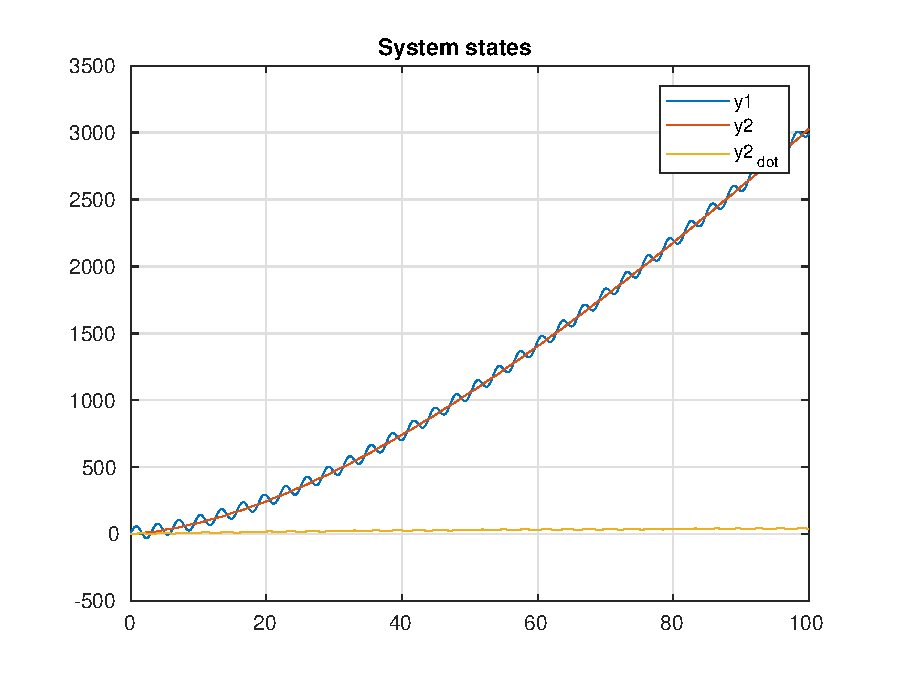
\includegraphics[width=0.5\textwidth]{sys}
\caption{System simulation}
\label{fig:sys}
\end{figure}
Notice how the $y_1$ and $y_2$ positions diverge. This is due to the constant component of the input. In a regular mass-spring-damper configuration, a spring is connected directly to the wall which will balance any constant applied force. When a damper is placed inbetween this spring an the wall on the other hand, it can in theory be stretched to infinity as damping force for a theoretical damper is only dependent on speed. As for the input, it should also be noted that the sine component has been scaled with a significantly higher gain (close to $100$) than the $5$ gain that was mentioned in the assignment. When the adaptive law from (4.4.5) is implemented, this results in parameter convergence as shown in figure \ref{fig:params} below.
\begin{figure}[H]
\centering
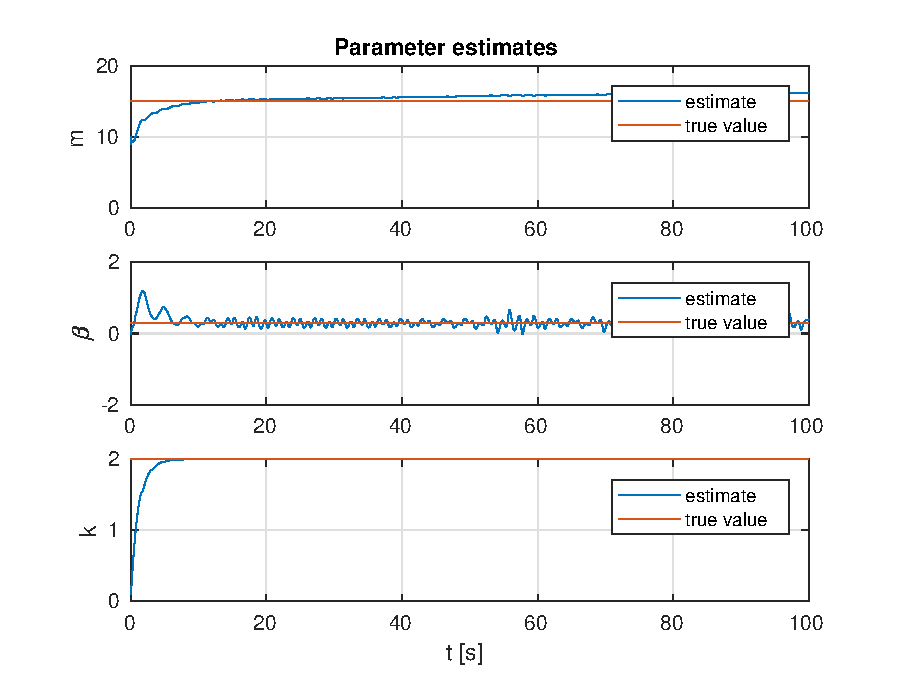
\includegraphics[width=0.6\textwidth]{params}
\caption{Parameter estimation}
\label{fig:params}
\end{figure}

\section{I\&S 4.11}
\subsection{}
Starting with $i=0$ we have for the first closed loop
\begin{equation}\begin{aligned}
\theta_p = G_0(r - \theta_o)
\end{aligned}\end{equation}
which yields
\begin{equation}\begin{aligned}
s^2 \theta_p &= k_0 \omega_0^2 (r-\theta_p)
-\omega_0^2(1-k_0)\theta_p
- 2 \xi_0 \omega_0 s \theta_p \\
&= k_0\omega_0^2 r - k_0 \omega_0^2 \theta_p - \omega_0^2 \theta_p + k_0 \omega_0^2 \theta_p - 2 \xi_0 \omega_0 s \theta_p \\
&=k_0 \omega_0^2 r - \omega_0^2 \theta_p - 2\xi_0 \omega_0 s \theta_p \\
&=
\begin{bmatrix}
k_0 \omega_0^2 & \omega_0^2 & \xi_0 \omega_0 \\
\end{bmatrix}
\begin{bmatrix}
r\\
-\theta_p\\
-2s\theta_p\
\end{bmatrix}
\end{aligned}\end{equation}
At this point we have something resenbling a parametrization, but to make the $s^2$ on the rhs realizable, we need to filter it with a second order stable filter. Choosing $\Lambda_0$ to be a second order Hurwitz polynomial in $s$ we get the parametrization $z_0 = \theta_0^{*\top}\phi$ with
\begin{equation}\begin{aligned}
z_0 = \frac{s^2 \theta_p}{\Lambda_0}, \quad
\phi_0 = \frac{1}{\Lambda_0}
\begin{bmatrix}
r\\
-\theta_p\\
-2s\theta_p \\
\end{bmatrix}, \quad
\theta_0^{*\top} =
\begin{bmatrix}
k_0 \omega_0^2\\
\omega_0^2 \\
\xi_0 \omega_0 \\
\end{bmatrix}.
\end{aligned}\end{equation}
From this we will find $\omega_0^2$, which lets us calculate the values of $k_0$ and $\xi_0$. For $i = 1$ the closed loop yields
\begin{equation}\begin{aligned}
\dot \theta = G_1 \theta_p
\end{aligned}\end{equation}
which becomes
\begin{equation}\begin{aligned}
s^2 \dot \theta &= k_1 \omega_1^2 \theta_p - 2 \xi_1 \omega_1 s \dot \theta - \omega_1^2 \dot \theta \\
&=
\begin{bmatrix}
k_1 \omega_1^2 & \omega_1^2 & 2 \xi_1 \omega_1
\end{bmatrix}
\begin{bmatrix}
\theta_p\\
-\dot \theta \\
- 2 s \dot \theta
\end{bmatrix}
\end{aligned}\end{equation}
Filtering with a filter with the same properties as $\Lambda_0$, we can obtain the parametrization $z_1 = \theta^{*\top}_1 \phi$ with
\begin{equation}\begin{aligned}
z_1 = \frac{s^2 \theta_p}{\Lambda}, \quad
\phi_1 = \frac{1}{\Lambda_1}
\begin{bmatrix}
\theta_p\\
-\dot \theta \\
- 2 s \dot \theta
\end{bmatrix}, \quad
\theta_1^{*} =
\begin{bmatrix}
k_1 \omega_1^2 \\
 \omega_1^2 \\
 2 \xi_1 \omega_1\\
\end{bmatrix}.
\end{aligned}\end{equation}
As with $i = 0$ we can here too solve for $k_1$ and $\xi_1$ using $\omega_1$.
\end{document}

